\documentclass[10pt]{exam}
\usepackage[phy]{template-for-exam}
\usepackage{graphicx}
\usepackage{enumitem}
\setlist{topsep=0pt,itemsep=-1ex,partopsep=1ex,parsep=1ex}

\title{Pendulum Lab Report Guidelines}
\author{Rohrbach}
\date{\today}

\begin{document}
\maketitle

\section*{Pre-Lab}


\begin{questions}



\question
  Recall the difference between independent, dependent, and control variables.
  \vs 

\question
  Brainstorm a list of factors that might affect the period of a pendulum.
  \vs 

\question
  Identify each of the following (there may be more than one).

  \begin{center}
    \begin{tabular}
      { m{.25\textwidth} | m{.3\textwidth}| m{.25\textwidth} } 
      Independent Variables & 
      Dependent Variables   & 
      Control Variables  \\[10em]
    \end{tabular}
  \end{center}

\end{questions}

\section*{Lab Report}
\emph{All of the your answers from here on should go in the word document.}

\paragraph{Purpose:} 
  Write one sentence explaining what you are trying to figure out in this lab. Make sure your purpose includes all of your independent and dependent variables

\paragraph{Hypotheses:} 
  Predict what the relationship will be between each of your independent variables and your dependent variable (\emph{i.e. directly proportional, inversely proportional, unrelated).} Make sure to explain why you think each of these relationships will hold.

  \emph{Example:} mass and period will be (choose one: directly proportional, inversely proportional, unrelated).


\paragraph{Procedure:} 
  Make a brief list of the steps you follow in the lab.

  \begin{itemize}
    \item
      Make a list of all three experiments that you will perform.
    \item
      Explain how, specifically, you will be measuring the dependent variable.
    \item
      Explain how many values of each independent variable there will be.

  \end{itemize}

\pagebreak

\paragraph{Data:}
  Show all data tables for each of your experiments.

  \begin{itemize}
    \item
      Be sure that each data table has a descriptive title.
    \item
      Be sure that each data table lists the variables you are holding constant and their values
    \item
      Make sure all units are labeled. (It is OK to label the units in the table headings instead of in each individual cell
    \item
      You'll probably have a total of \textbf{three} data tables in your report (one for each independent variable)
    \item
      Each data table should have 5 different rows (one for each value of the independent variable)
  \end{itemize}

  \noindent
  \begin{minipage}[b]{4.4in}
    \noindent
    Also include a Desmos graph for each variable
  
    \begin{enumerate}
      \item
        Go to \texttt{www.desmos.com/calculator} to graph your data.
      \item 
        Make a separate graph for \emph{each} expeiment.
      \item
        Graph your independent variable on the $x$-axis and dependent variable on the $y$-axis
      \item
        Use the ``wrench icon'' to give your graph axis labels.
      \item 
        Make sure to zoom your graph in such a way that your data fills the page \emph{and} that you can see zero on each axis.
      \item
        Copy the share link (top image to the right).
      \item
        Also, click ``Export image.'' Right click the graph and then click ``Copy image'' (bottom image to the right). Paste into your data
        table.
    \end{enumerate}
  \end{minipage}
%
  \begin{minipage}[t]{2in}
    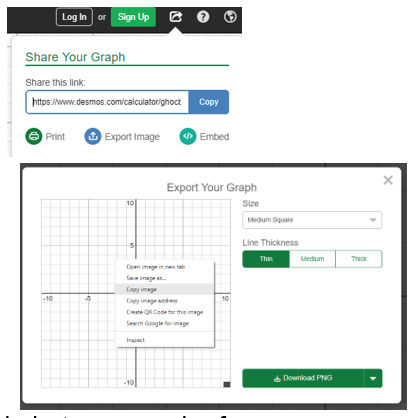
\includegraphics[width=2in]{desmos.png}
  \end{minipage}

  


\paragraph{Results:} 
  All you need are three sentences for this section: one for each experiment.  Your results should describe the relationship between each of your independent variables and your dependent variable (\emph{i.e. directly proportional, inversely proportional, unrelated)}.
    
  \emph{Example:} Mass and period were unrelated.

\paragraph{Conclusion and Discussion:}
  Answer the following questions in paragraph form.

  \begin{itemize}
    \item
      What was the purpose of the lab?
    \item
      How did you go about accomplishing the purpose?
    \item
      What did you find (\emph{i.e.} what affected the period of the
      pendulum and how did it affect it)?
    \item
      What errors came up in this lab and how could you correct them in the
      future?
  \end{itemize}

\end{document}